\section{Kinematics and Timing of Signal and Background events}
\label{sec:kinematics_and_timing}

\subsection{0\nbb-decay signal and 2\nbb-decay background}

In both 0\nbb-decay signal and 2\nbb-decay background events near the decay energy spectrum endpoint, the kinematics of the
electron pair is very similar. Large fraction of events have a nearly back-to-back topology with a close to 
equal energy split between electrons. To simulate 0\nbb- and 2\nbb-decay events we use a Monte Carlo generator based on phase 
factors from Ref.~\cite{Jenni}. Similarity in kinematics of 0\nbb- and 2\nbb-decay events is demonstrated in Fig.~\ref{fig:Kinematics}.

The electron angular correlations for 0\nbb-decay are noticeably different from 2\nbb-decay due to a contribution from
neutrinos wave-function even at vanishingly small energies of the neutrinos~\cite{Jenni}. However, any practical use of this difference 
in separating 0\nbb-decay from 2\nbb-decay would require extremely large number of candidate events. Given half-time of 2\nbb-decay 
and upper limits on the half-time of 0\nbb-decay, electron angular correlations won't bring decisive separation power in controlling 
2\nbb-decay background in currently planned 0\nbb-decay experiments. Excellent energy resolution at the Q-value is the key parameter
in 2\nbb~background suppression.

While we don't exclude that the angular correlations as an input to a multivariative technique may improve sensitivity of 0\nbb-decay 
searches, in this paper we assume that there is no difference in the event topology between 0\nbb-~and 2\nbb-decay events. Any conclusions 
about 0\nbb-decay events also hold for 2\nbb-decay when total energy of the electrons in 2\nbb-decay events is close to the Q-value.


\begin{figure*}[ht]
  \centering
  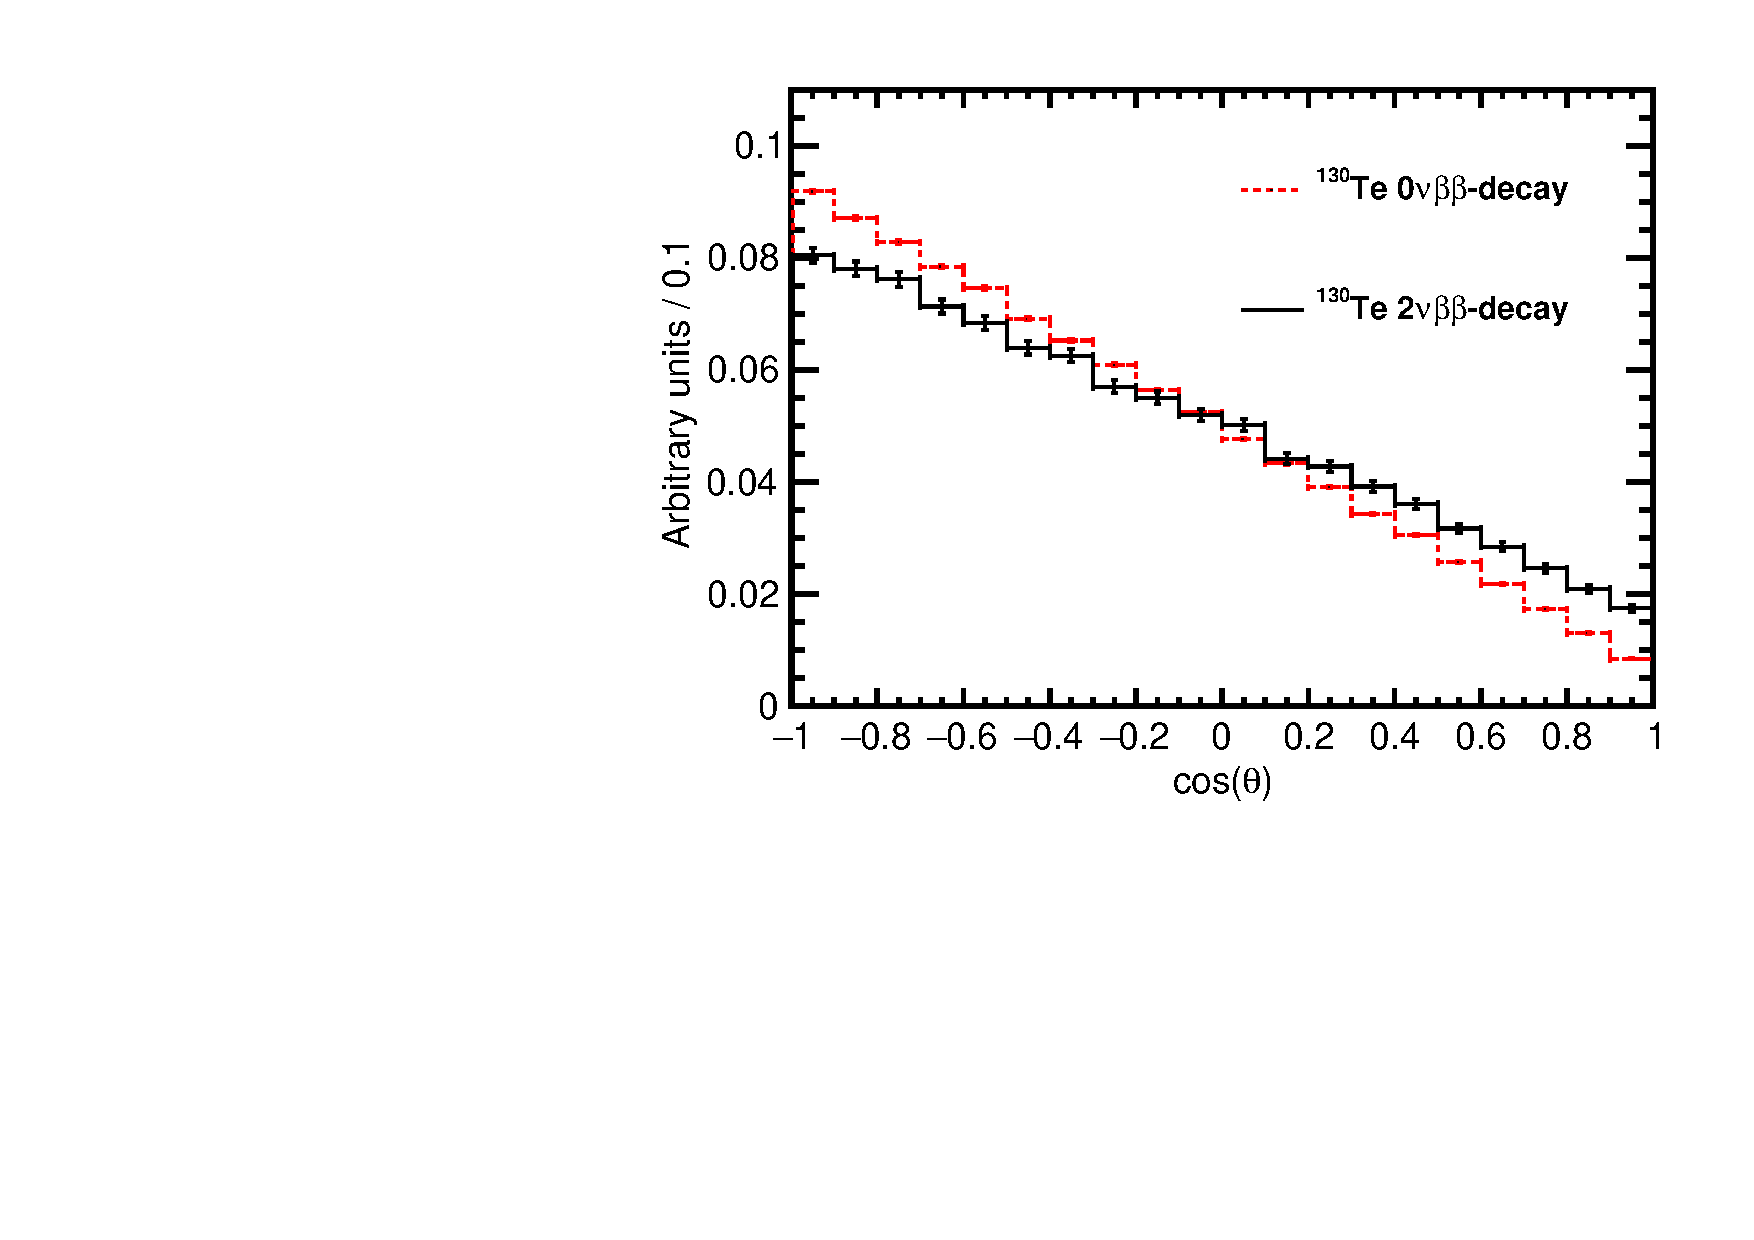
\includegraphics[width=0.49\textwidth]{hCos_Te130.pdf}
  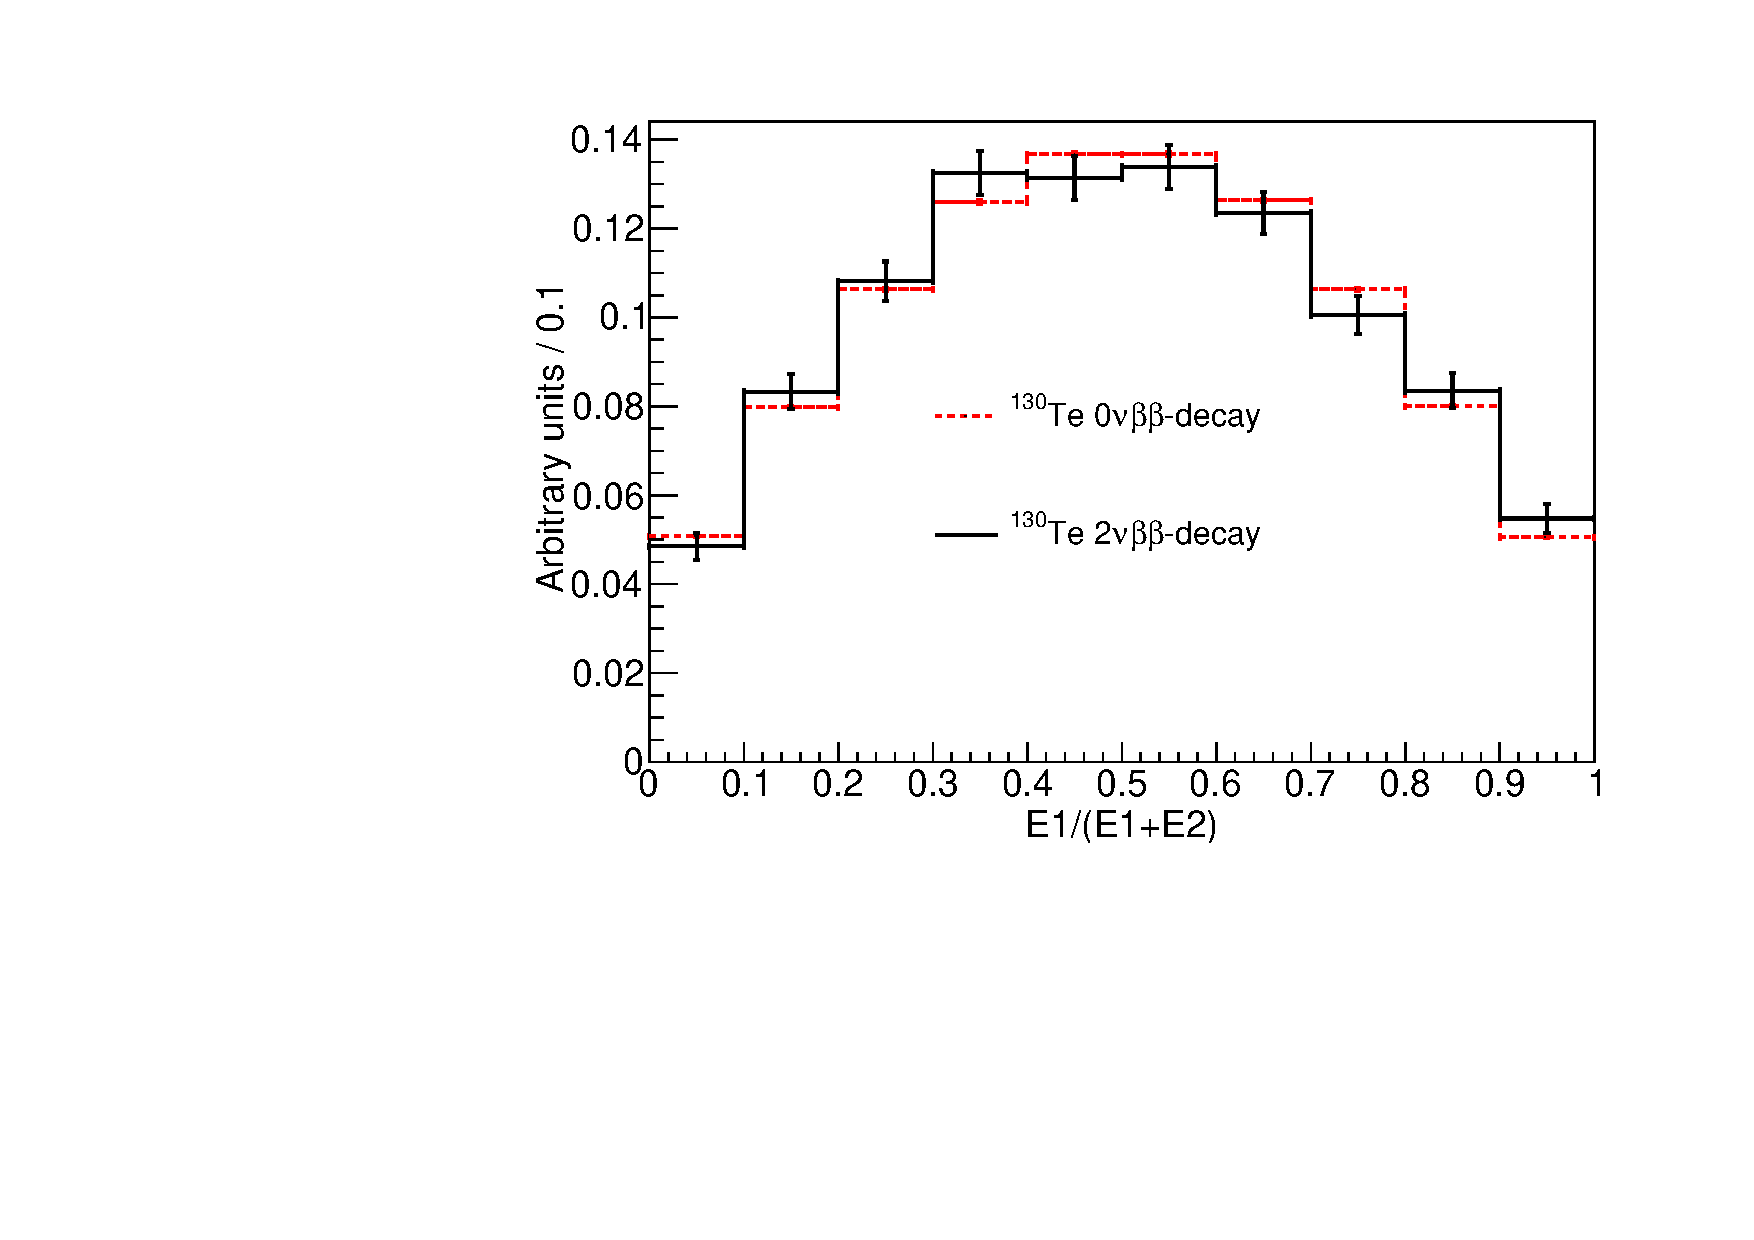
\includegraphics[width=0.49\textwidth]{hE1toQ_Te130.pdf}
  \caption{Comparison between kinematics of 0{\nbb} (\emph{dashed red
      lines}) and 2{\nbb} decays (\emph{solid black lines}) for events
    with the total kinetic energy of the electrons above 90\% of the
    Q-value. \emph{Left:} Cosine of the angle between two
    electrons. \emph{Right:} Fraction of energy carried by one of the
    two electrons. Vertical bars at each bin of the histograms indicate
    statistical uncertainty for that bin.}
  \label{fig:Kinematics}
\end{figure*}


%Should we recalculate for 130Te.
Examining the kinematics for one of the 0\nbb~electrons with equal energy split, a 1.26~MeV electron travels a total path length of 0.X~cm, 
has a distance from the origin of 0.X~cm in 0.0X$\pm$0.00X~ns  and takes 0.0X$\pm$0.00X~ns to drop below Cherenkov threshold. 
We note that due to scattering of the electron, the final direction of the electron before it stops does not correspond to the initial 
direction; however the scattering angle is small while the majority of Cherenkov light is produced.

Figure~\ref{fig:ArrivalTimeDist} shows the output of the detector simulation for 1000 simulated \Te~ 0\nbb-decay 
events. The left panel in Fig.~\ref{fig:ArrivalTimeDist} compares PE arrival time between Cherenkov and scintillation light  
and the right panel in Fig.~\ref{fig:ArrivalTimeDist} zooms in on the Cherenkov photon distribution which is key to direction and 
topographical reconstruction.


\begin{figure*}[ht]
  \centering
  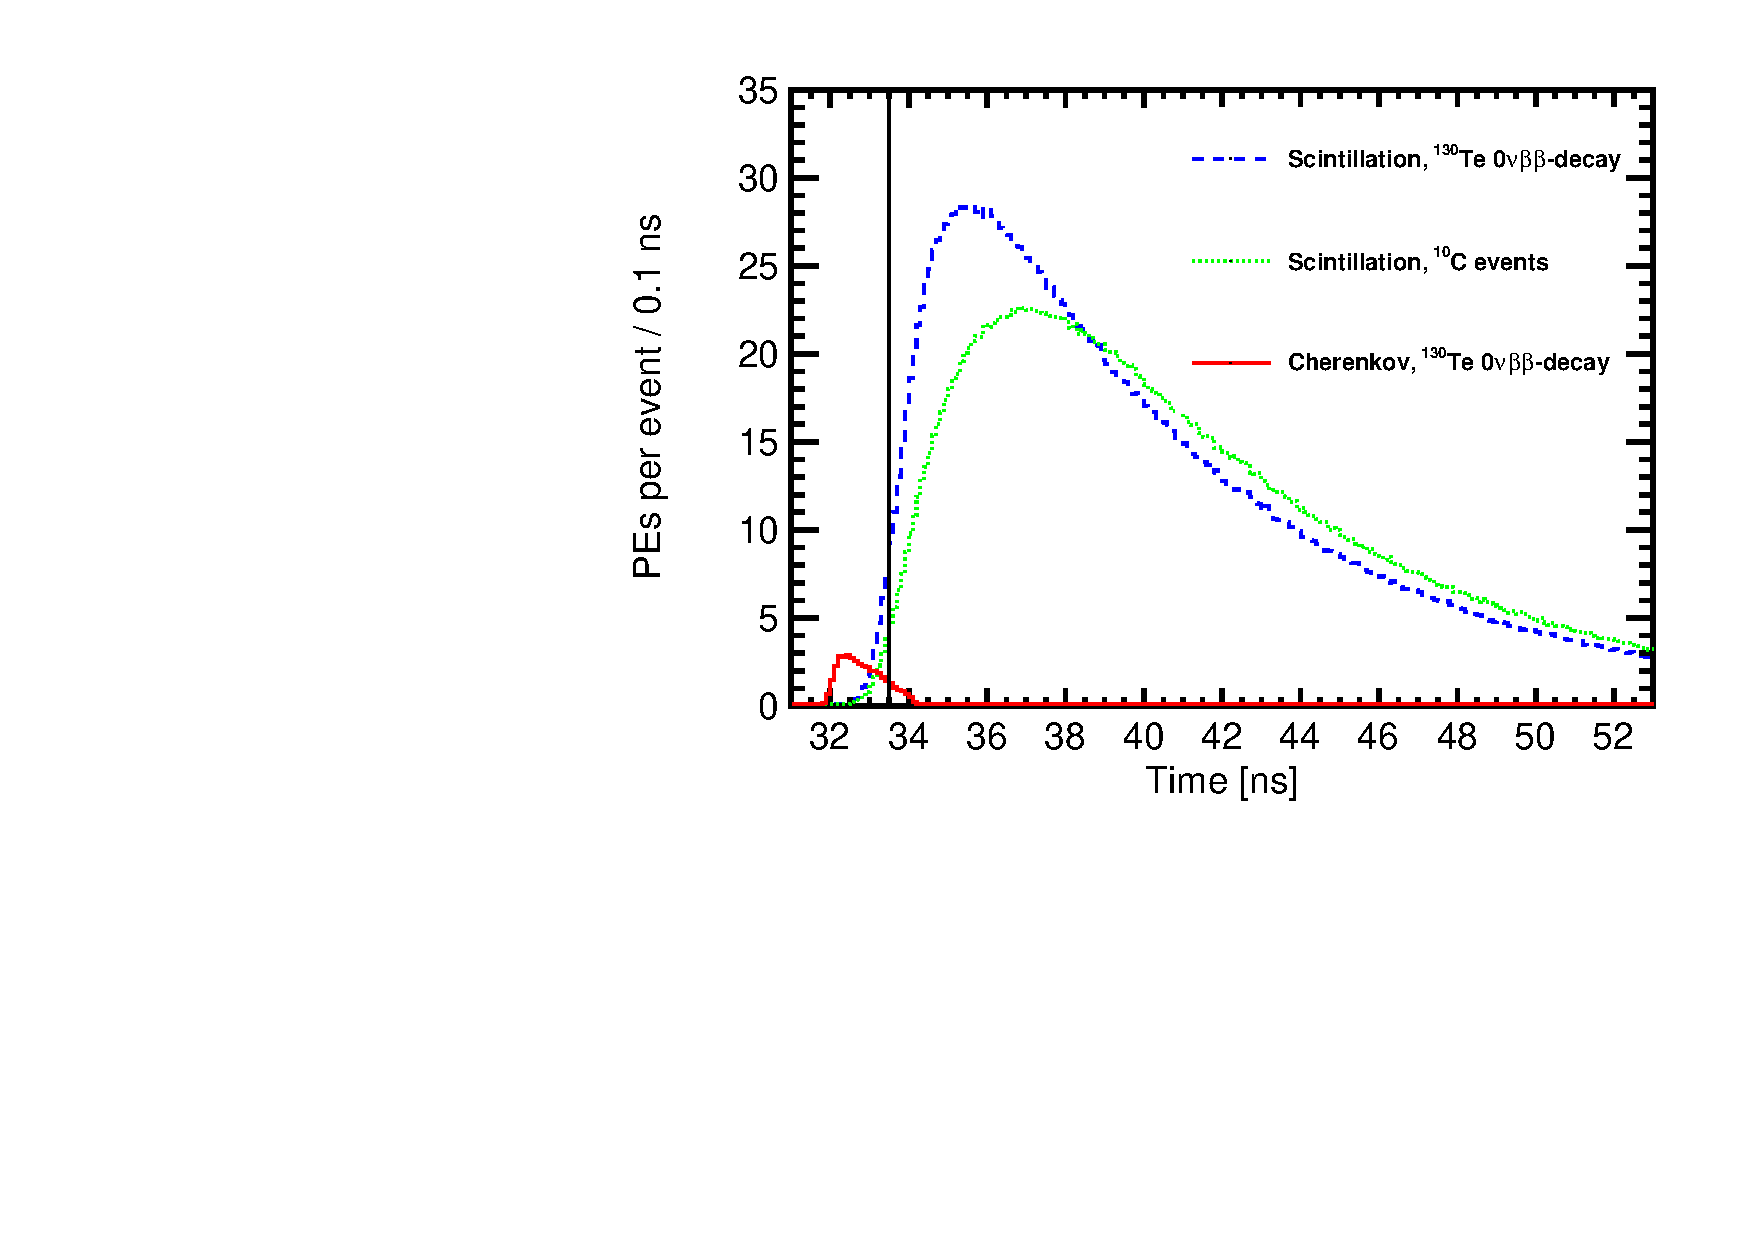
\includegraphics[width=0.45\textwidth]{hT_scintillation.pdf}
  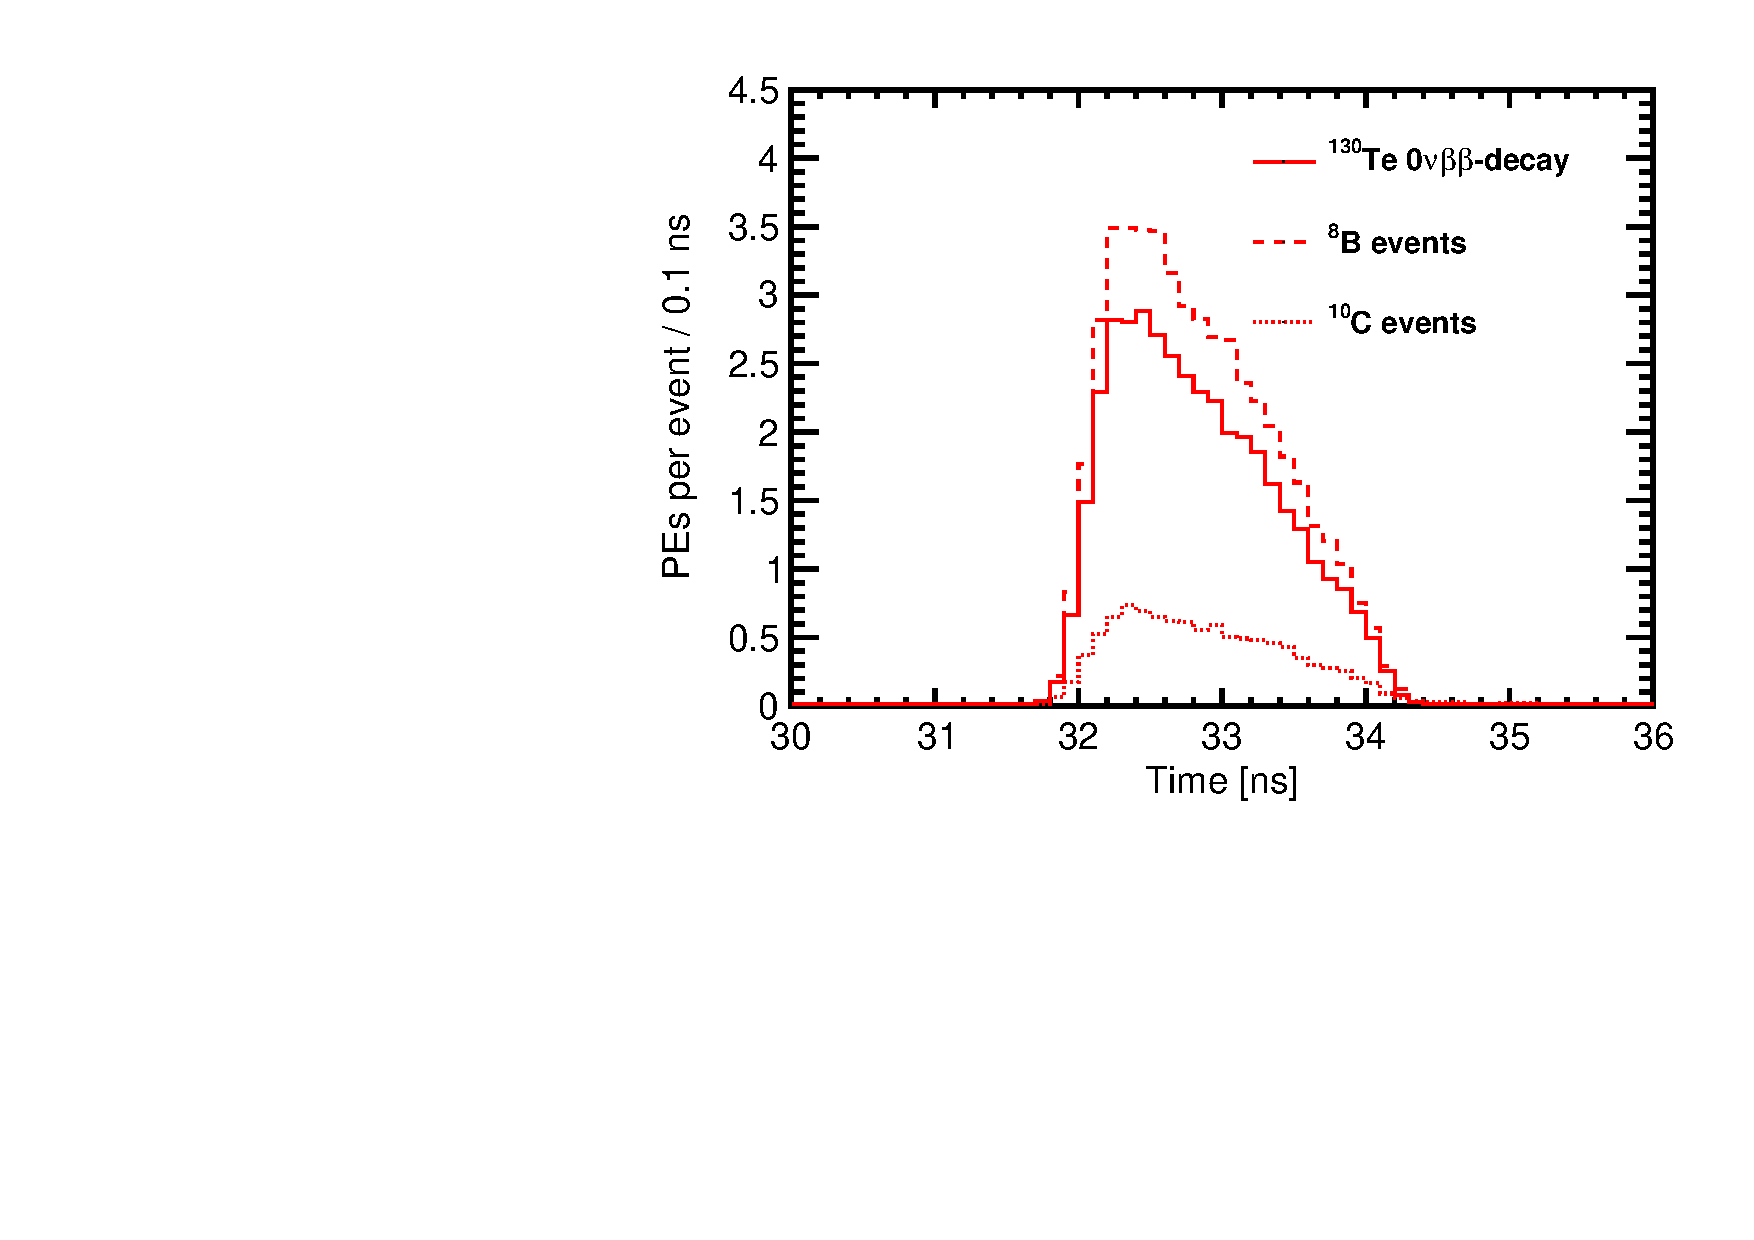
\includegraphics[width=0.45\textwidth]{hT_cherenkov.pdf}
  \caption{\emph{Left:} Photo-electron (PE) arrival times after
    application of the photo-detector transit time spread (TTS) of 100~ps for the default simulation 
    of \Te~0\nbb-decay and \C~events produced at the center of the detector. 
    Scintillation PE arrival time distribution is compared for \nbb-decay (dashed blue line) and
    \Cten~events (dotted green line). The corresponding distribution for \B~events is not shown
    because it is indistinguishable from the distribution for \nbb-decay. Cherenkov PE arrival
    times are shown for \nbb-decay (\emph{solid red line}) to demonstrate their contribution to the early PE sample.
    The vertical line at 33.5~ns indicates the time cut for the selection of the early PE sample.
    The shape of scintillation PE arrival times for \B~events
    \emph{Right:} Comparison between Cherenkov PEs arrival time for \Te~0\nbb-decay (\emph{solid line}), 
    \B~(\emph{dashed line}), and \C~events (\emph{dotted line}).}
\label{fig:ArrivalTimeDist}
\end{figure*}


Selection of PEs with relatively small arrival time allows to select a sample of PEs with high fraction of directional Cherenkov light.
This allows for event topology reconstruction. In particular, signal-like events with exactly two electrons can be separated from events 
with only one electron such as from \B~solar neutrino interactions.

As shown in Fig.~\ref{fig:ArrivalTimeDist}, for events produced at the center of the detector, a time cut of 33.5~ns on the PE arrival 
time selects a sample of early PEs that includes the majority of directional Cherenkov photons. Scintillation PEs also are 
selected with this time cut. Figure~\ref{fig:NPhotDist} shows the total number of scintillation and Cherenkov PE per event in the early 
PE sample for signal and background events.



\begin{figure*}[ht]
  \centering
  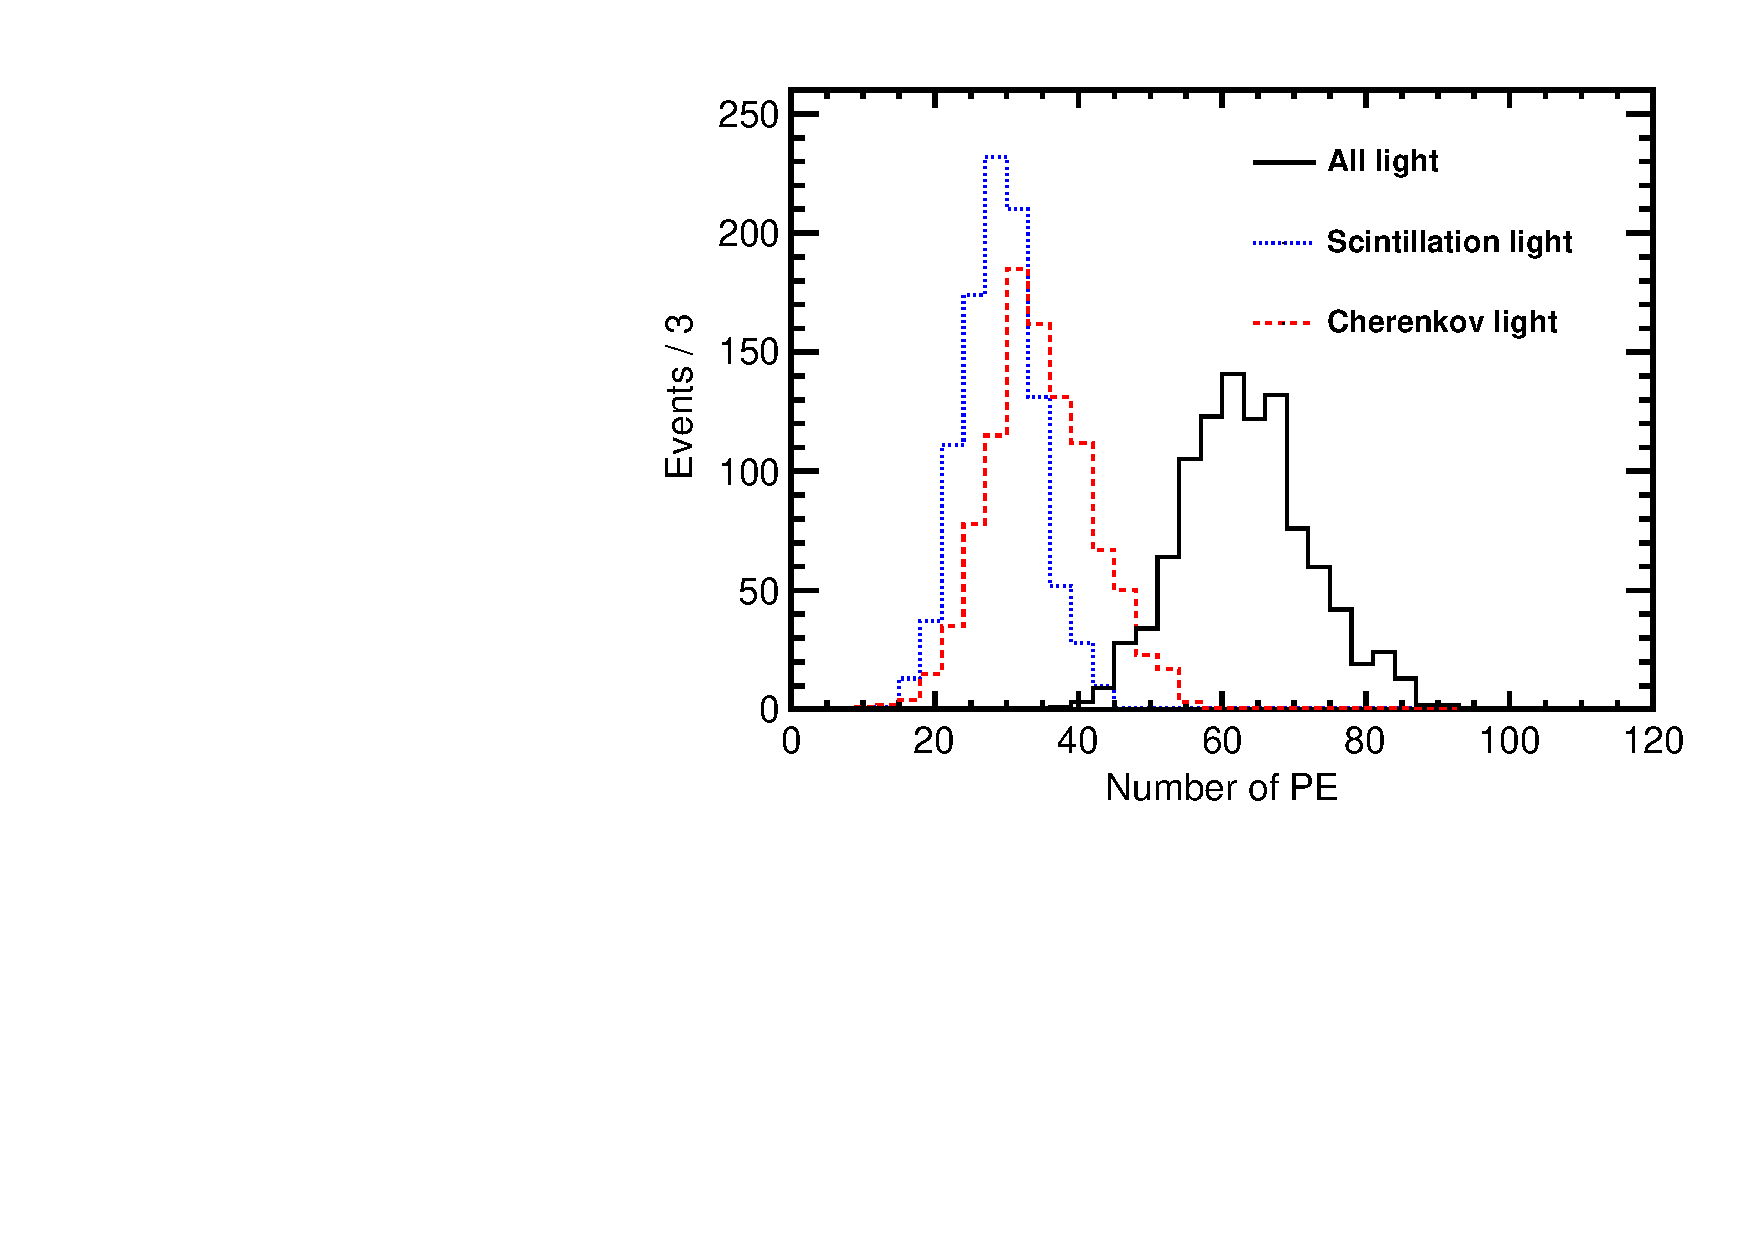
\includegraphics[width=0.33\textwidth]{hMomNPhot_Te130.pdf}
  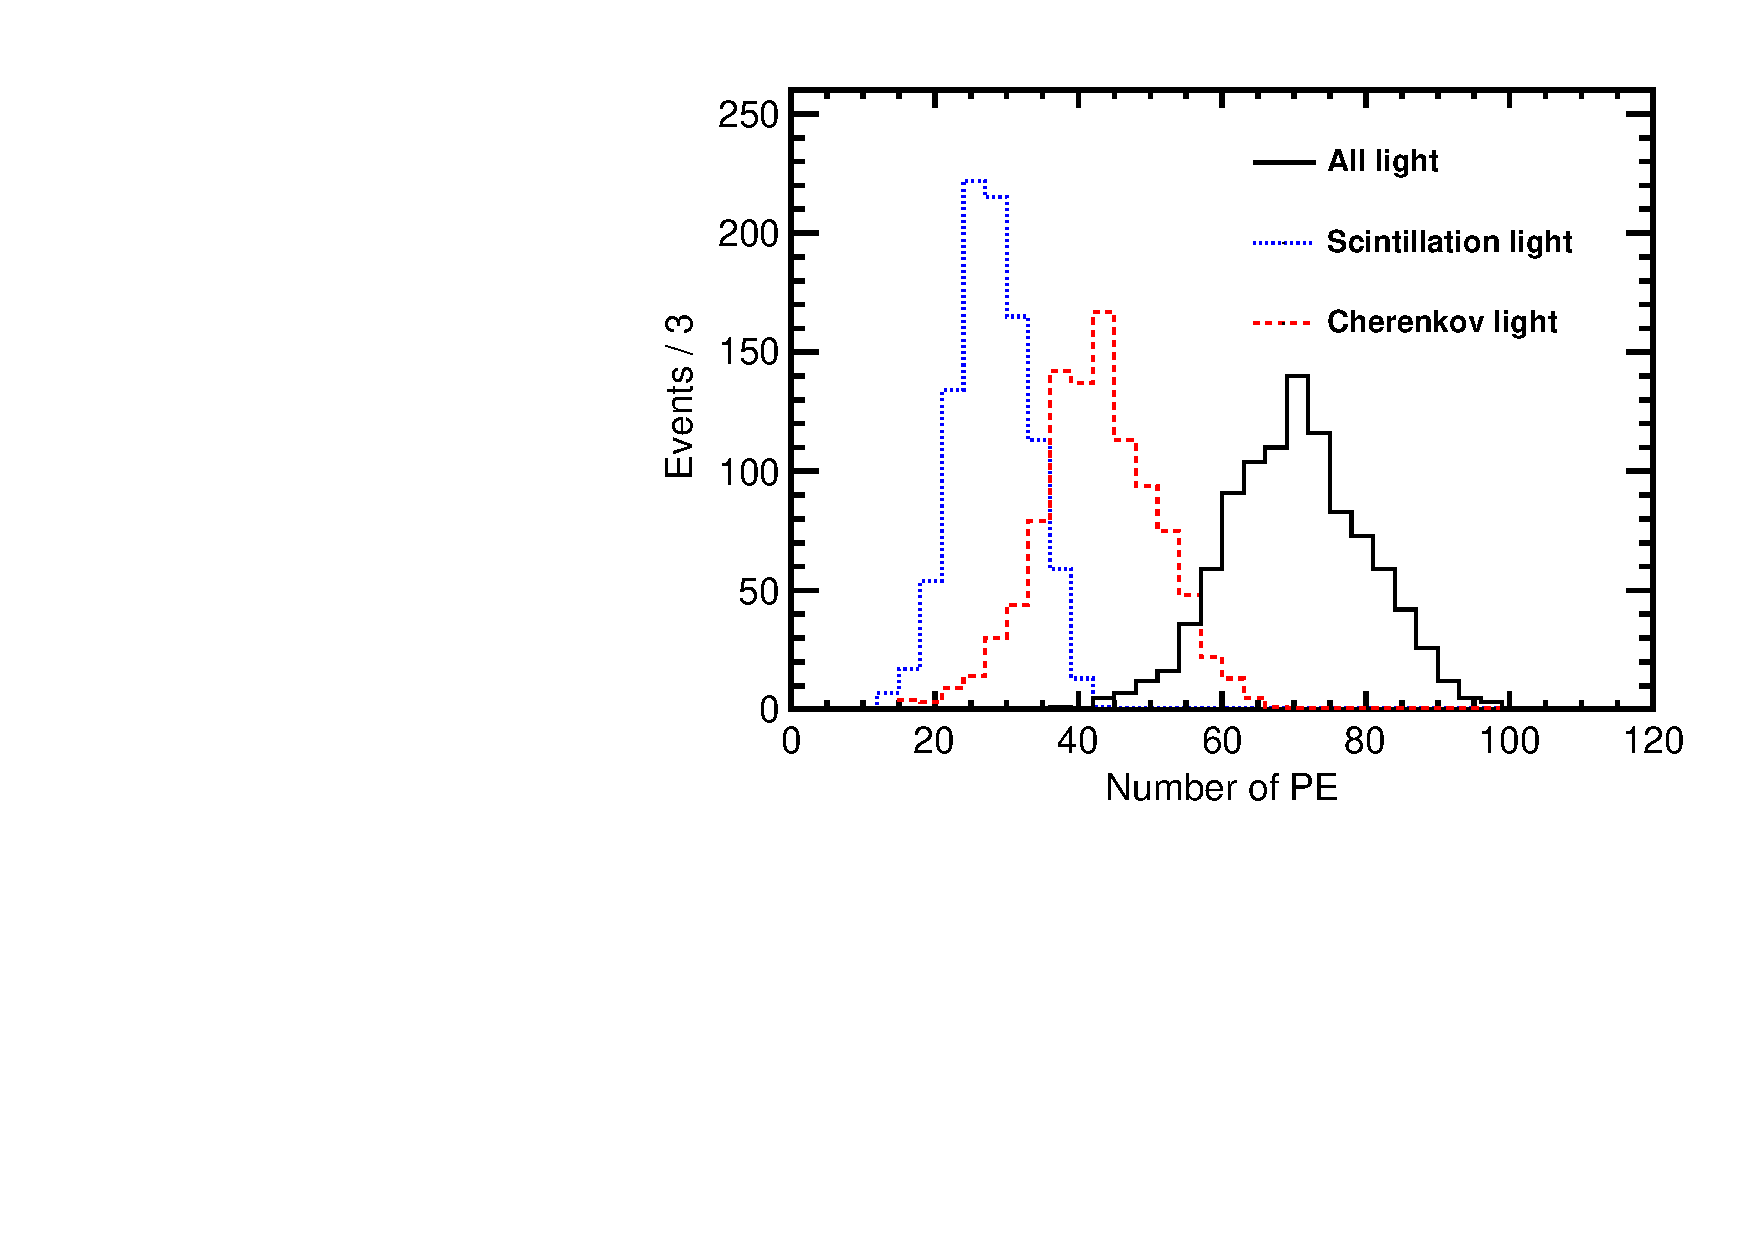
\includegraphics[width=0.33\textwidth]{hMomNPhot_1el_2p529MeV.pdf}
  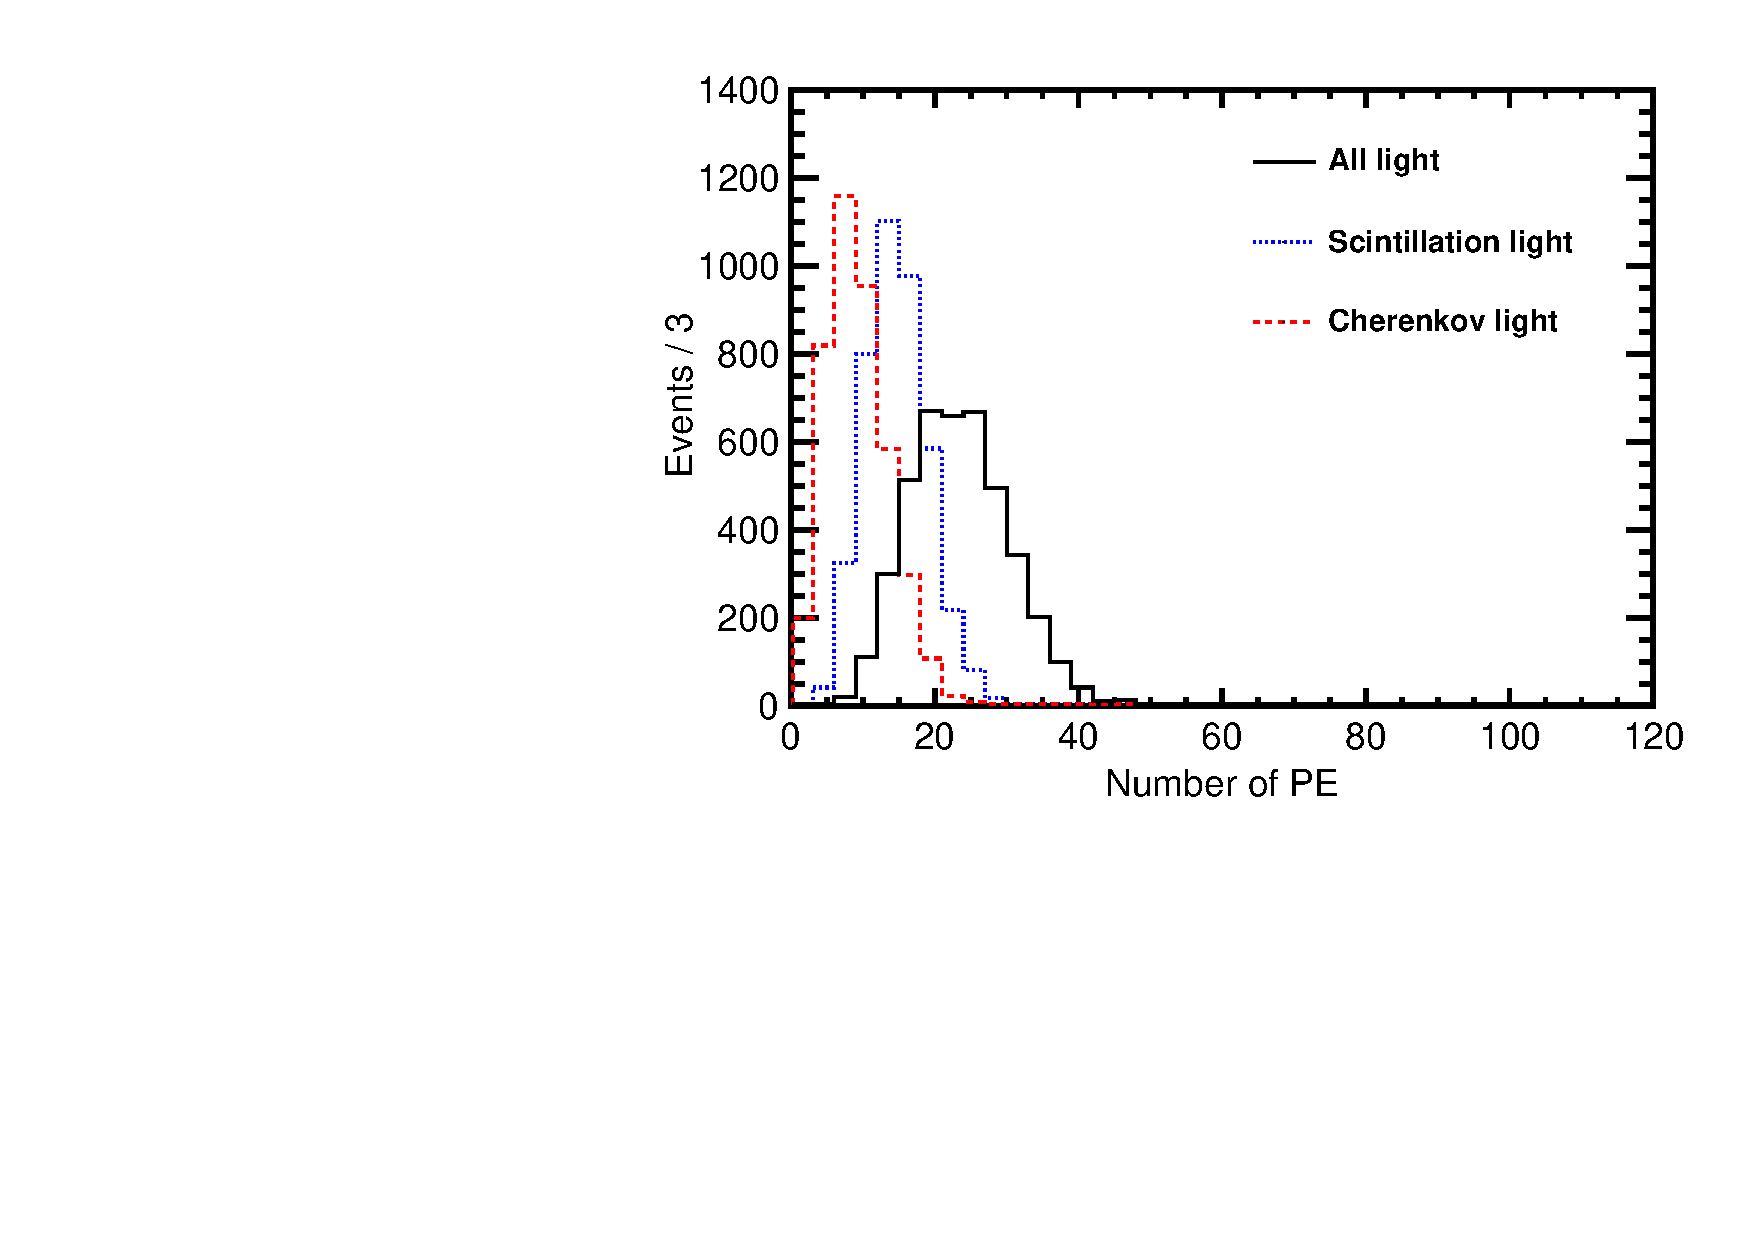
\includegraphics[width=0.33\textwidth]{hMomNPhot_C10.pdf}
  \caption{Early PE sample composition: number of Cherenkov (\emph{dashed red line}), scintillation
    (\emph{dotted blue line}), and total (\emph{solid black line}) PEs per event
    for the simulation of 1000 $^{130}$Te 0\nbb-decay events (\emph{left panel}),
    1000 $^8$B events (\emph{middle panel}), and 4152 \C~events (\emph{right panel}).}
\label{fig:NPhotDist}
\end{figure*}



\subsection{\B~background}

For a detector similar to our model \B~background is significant due to large mass.

Electrons from elastic scattering of \B~solar neutrinos have nearly flat energy spectrum around the 
Q-value~\cite{SNOp-B8-bkg}. We simulate \B~background as a single monochromatic electron with energy of 2.53~MeV 
(Q-value of \Te). A 2.53~MeV electron travels a total path length of 0.X~cm, has a distance from the origin of 0.X~cm in 
0.0X$\pm$0.00X~ns  and takes 0.0X$\pm$0.00X~ns to drop below Cherenkov threshold.

The scintillation PE timing distribution is unchanged compared to 0\nbb-decay since the electron's path lengths at these energies 
are too short to affect the effective vertex of the scintillation light. The number of Cherenkov photons is increased 
(see Fig.~\ref{fig:ArrivalTimeDist} and~\ref{fig:NPhotDist}) due to the increased electron kinetic energy but this alone is not 
sufficient to distinguish \B~events from 0\nbb-decay. However, it may provide an extra handle on signal-background separation in 
combination (e.g. by using multivariative techniques) with other event parameters.



\subsection{\C~background}

Background from \C~could be significant at a shallow detector depth.
Decay scheme of \C~is shown in Fig.~\ref{fig:C10_scheme_and_edep}. We note that 98\% of $^{10}$C decays through an excited state of $^{10}$B(718),
which has an unusually long half-life time of $\sim$1~ns. Therefore the majority of $^{10}$C events have a prompt positron accompanied by 
a delayed 0.718~MeV gamma. Because of the exponential nature of the delay, there will be still many \C~events where the delay in 
0.718~MeV gamma production won't be detectable due to finite time resolution of the detector. However photo-detectors with TTS below 100~ps, 
may allow for exploiting this delayed gamma for extra signal-background separation in some fraction of \C~events.

\begin{figure}[ht]
  \centering
  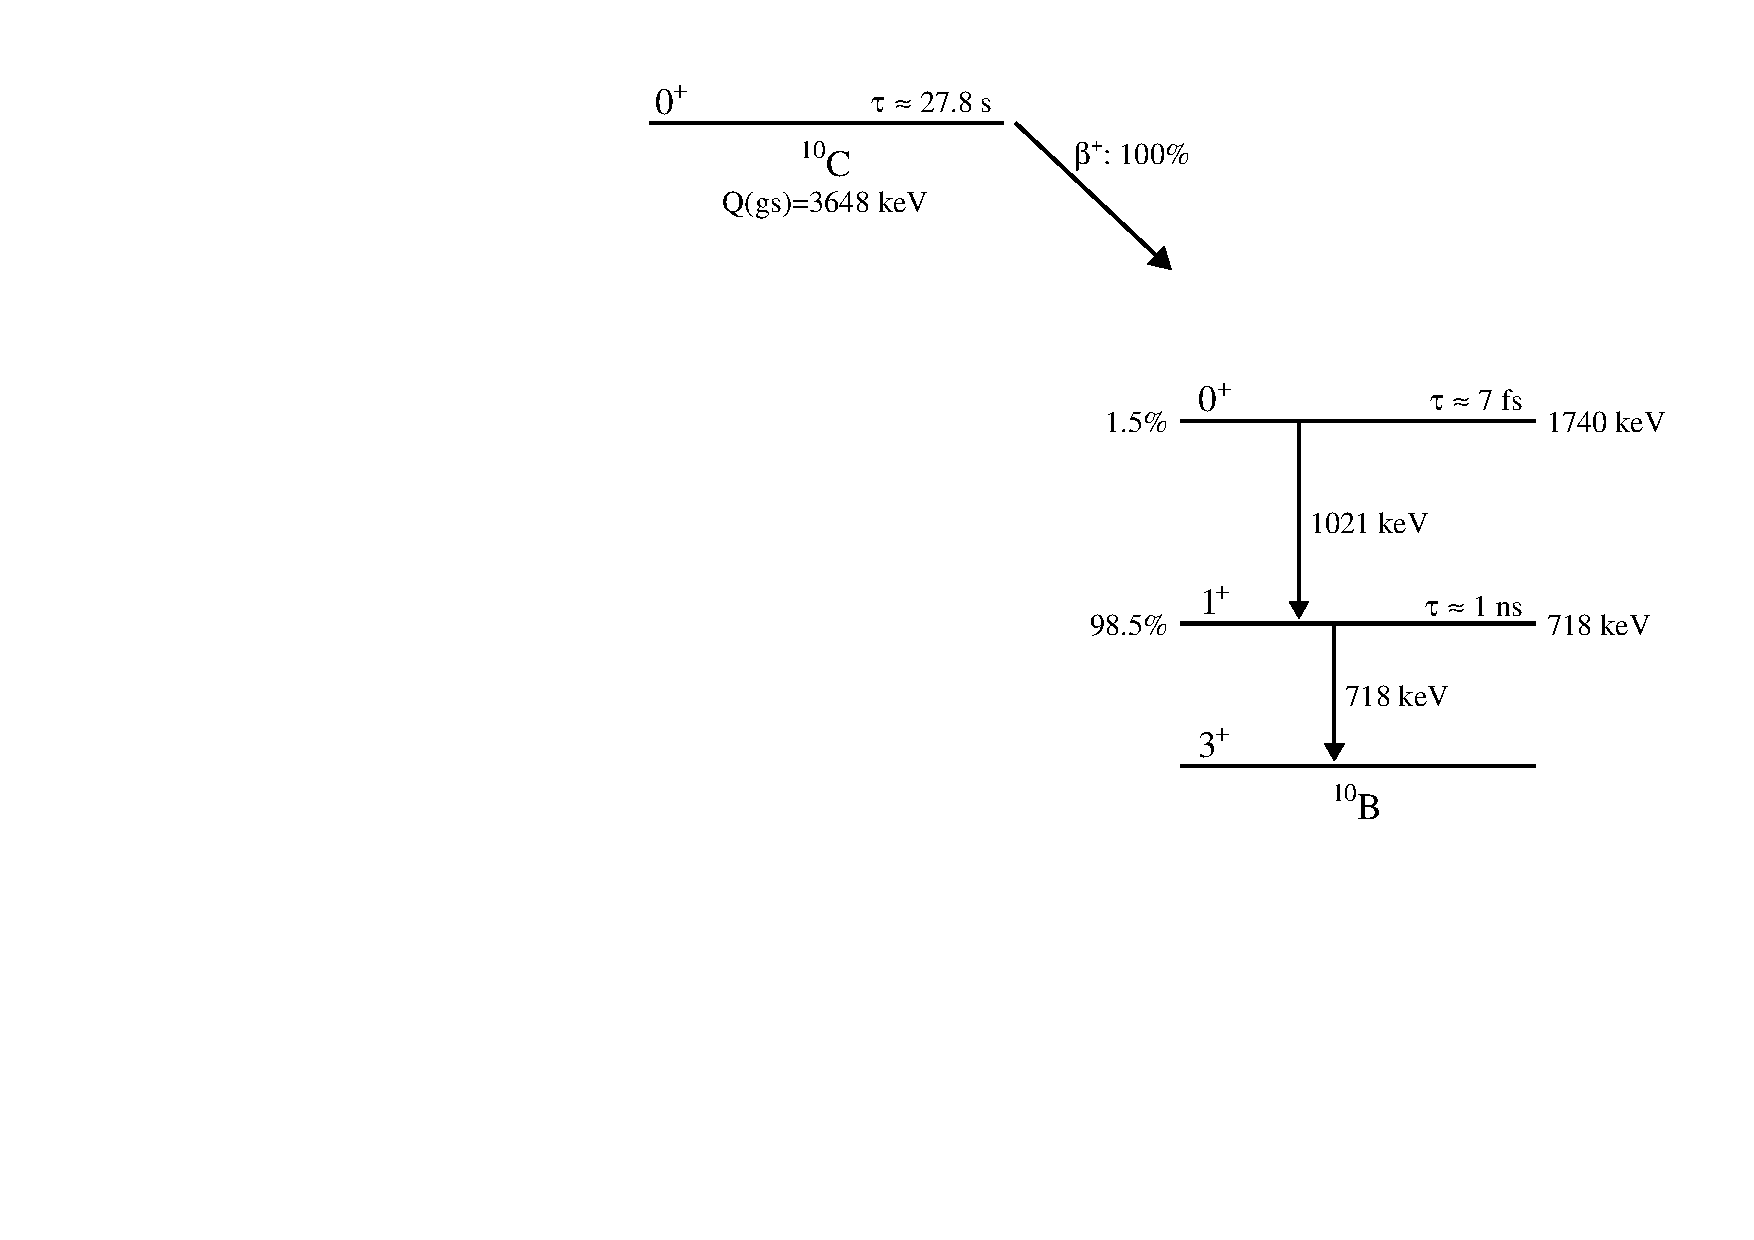
\includegraphics[width=0.49\columnwidth]{C10DecayScheme.pdf}
  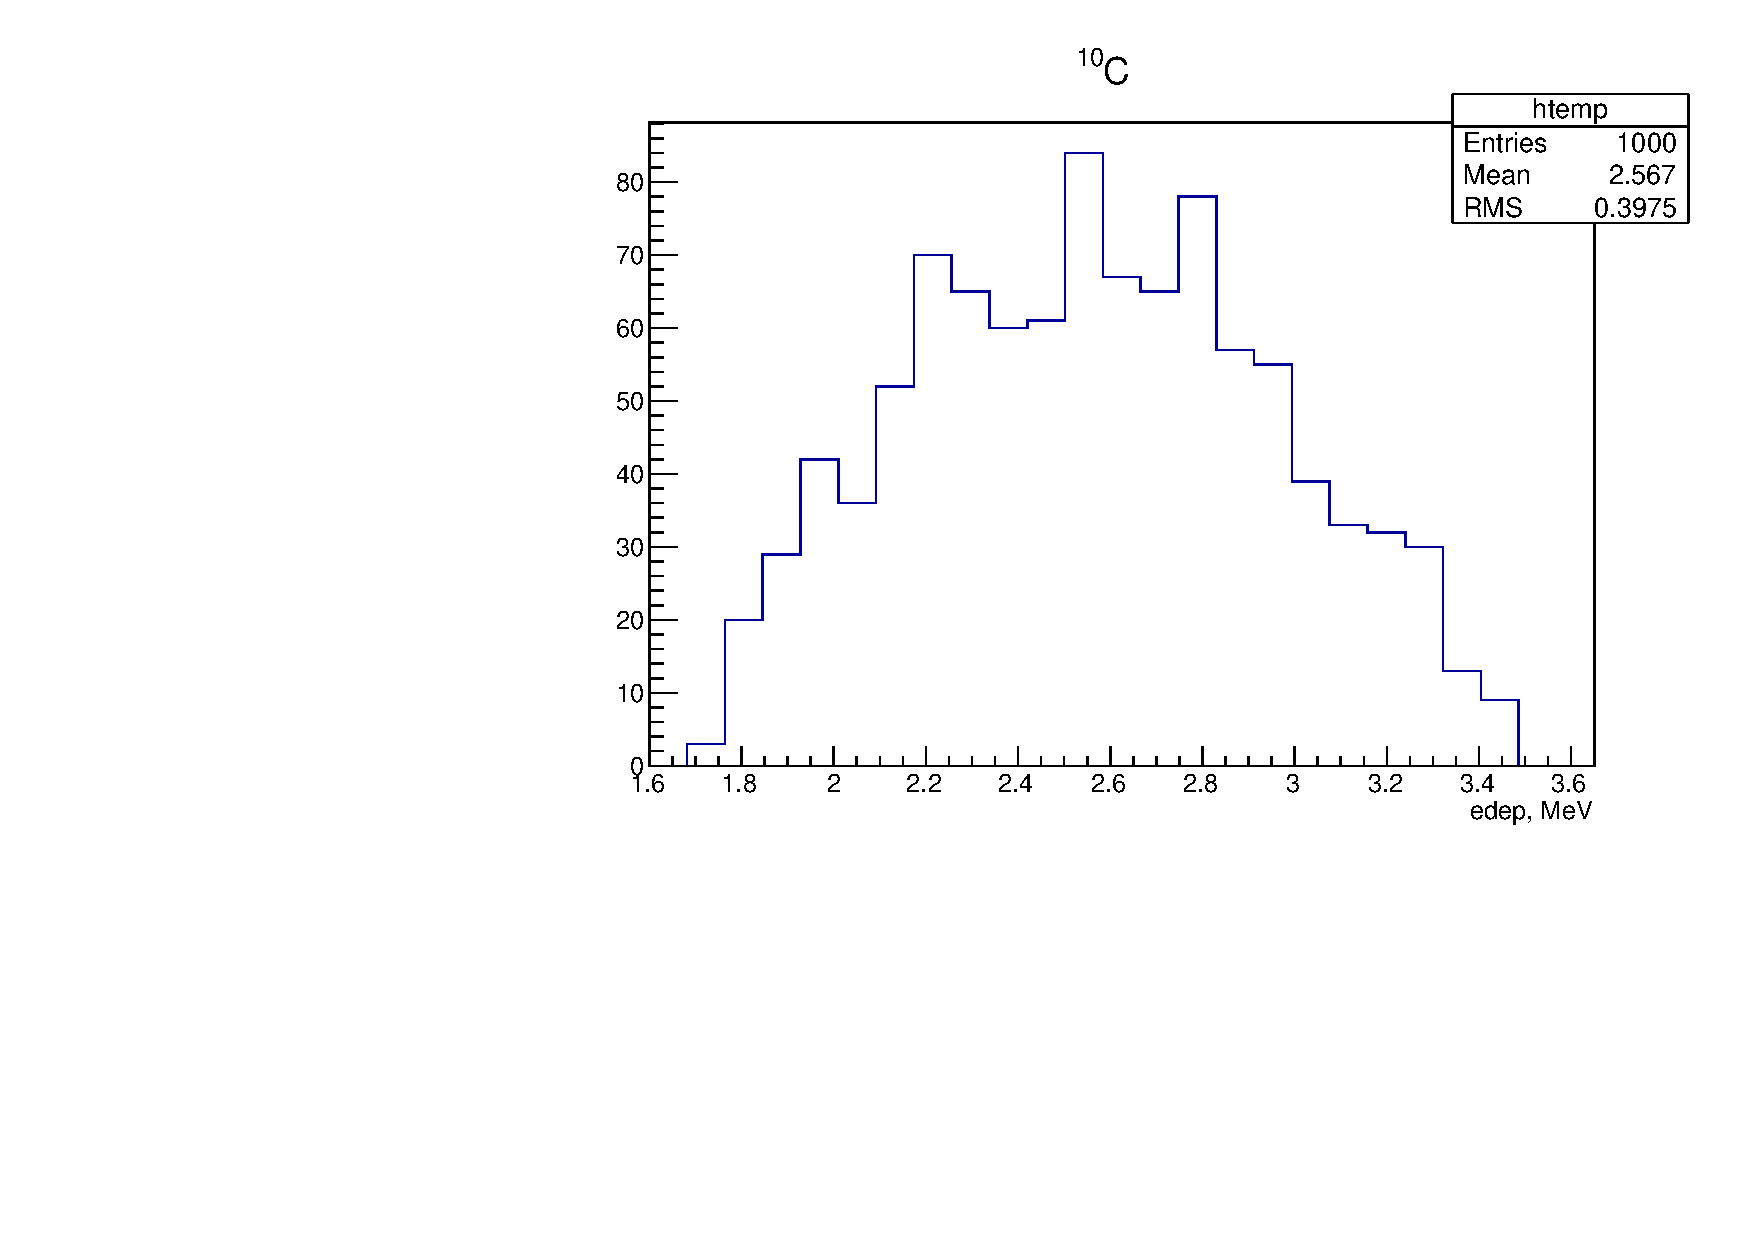
\includegraphics[width=0.49\textwidth]{hEdep_C10.pdf}
  \caption{\emph{Left:} Decay scheme of \C~events. \emph{Right:} Energy deposition in \C~events. Vertical solid line indicates 2.53~MeV
    which corresponds to Q-value of \Te~isotope. Vertical dashed lines indicate 2.28~MeV and 2.78~MeV corresponding to $\pm$10\% region 
    around the Q-value of \Te~0\nbb-decay.}
\label{fig:C10_scheme_and_edep}
\end{figure}

The energy of the positron in \C~events has to be 0.79~MeV for energy deposition to be equal to Q-value of \Te. Such positron on average 
travels 4~mm before it stops and annihilates producing two 0.511~MeV gammas or before it forms a (ortho-)positronium which in turn annihilates 
in two or three gammas. In a typical liquid scintillator there is about 50\% chance for a positron to form an ortho-positronium. 
An ortho-positronium in a liquid scintillator has a life-time of $\sim$3~ns~\cite{Ortho-positronium}. This delay in ortho-positronium annihilation
may significantly affect overall PE time distribution for \C~events. In some cases this alone allows for \C~background suppression, 
with photo-detectors time resolution being the major limiting factor in the signal-background separation efficiency~\cite{KLZ-use-of-PSD}.

Geant-4 simulation package, a standard tool for detector simulation, does not include simulation of ortho-positronium production and
annihilation~\cite{Geant4-release-and-private-communication}. Therefore our default detector model simulate $\sim$50\% of \C~events which
have ortho-positronium as an intermediate state. In the following we decided to leave such events with ortho-positronium out of discussion 
and focus on properties of the rest of \C~events that are more challenging to suppress.

The kinetic energy of the positron from \C~is smaller than total kinetic energy of the electrons from 0\nbb-decay. Therefore less 
Cherenkov and scintillation PEs are produced at the primary vertex. One 0.718~MeV from $10$B excited state and two 0.511~MeV gammas
from positron annihilation travel for about one radiation length while loosing their energy via Compton scattering and photo-electric effect.
Most of scintillation PEs in \C~events is produced at spatially separated secondary verticies which leads to significant smearing in scintillation 
PEs arrival time compared to 0\nbb-decay events where the scintillation is localized at the primary vertex (see Fig.\ref{fig:ArrivalTimeDist}). 
We note that this smearing is characteristic of any background that includes a positron as it would always be accompanied by at least 
two gammas.

Small number of Cherenkov PE can also be produced by low energy electrons at gamma interaction points, but it is hard to separate them
from scintillation PE due to uncertainties on the vertex position and time of each gamma interaction.



%\subsection{0\nbb/\C~separation using PE timing}
%\begin{figure}[h]
%  \centering
%  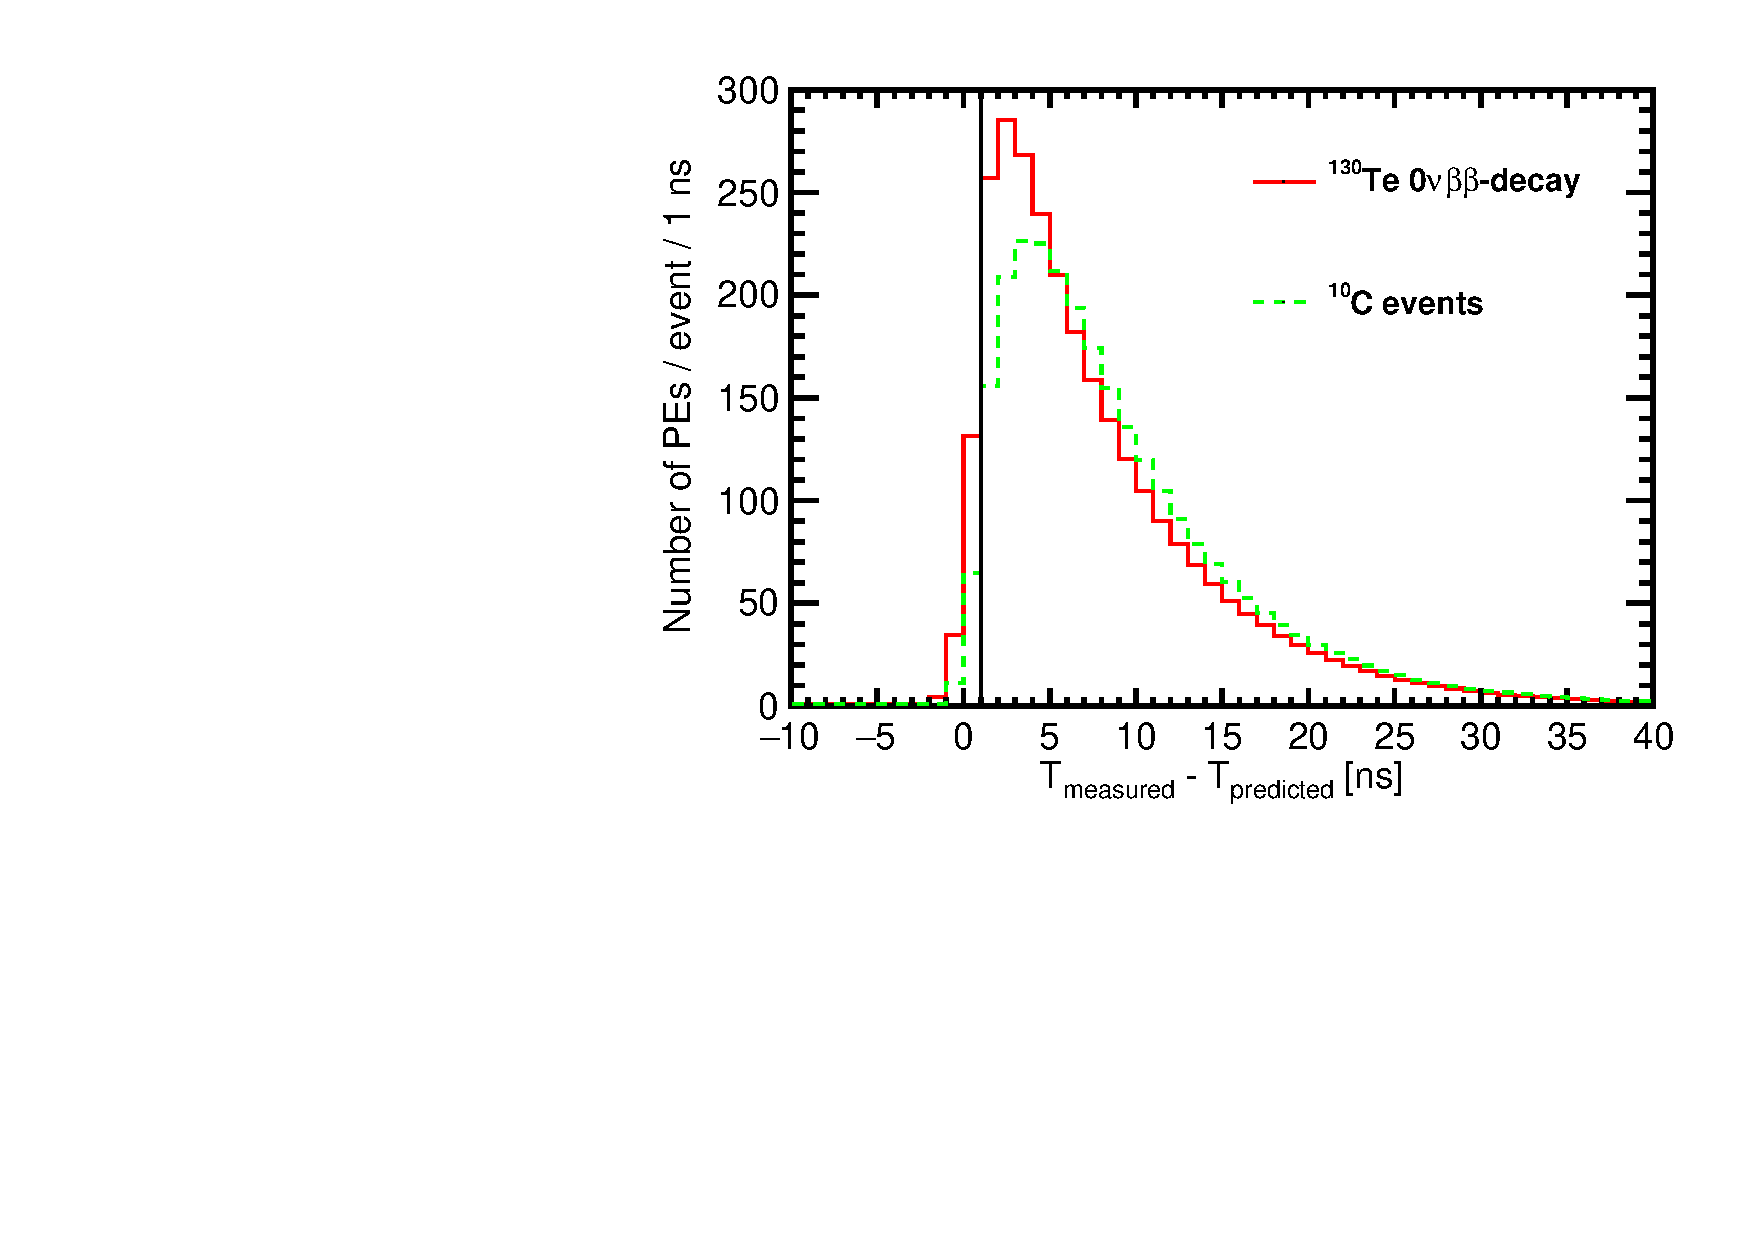
\includegraphics[width=0.45\textwidth]{hMomDT_Te130vsC10_allLight_VtxSmear3cm_VtxShiftX0cm_momDT1p0ns_rndVtx_3p0mSphere.pdf}
%  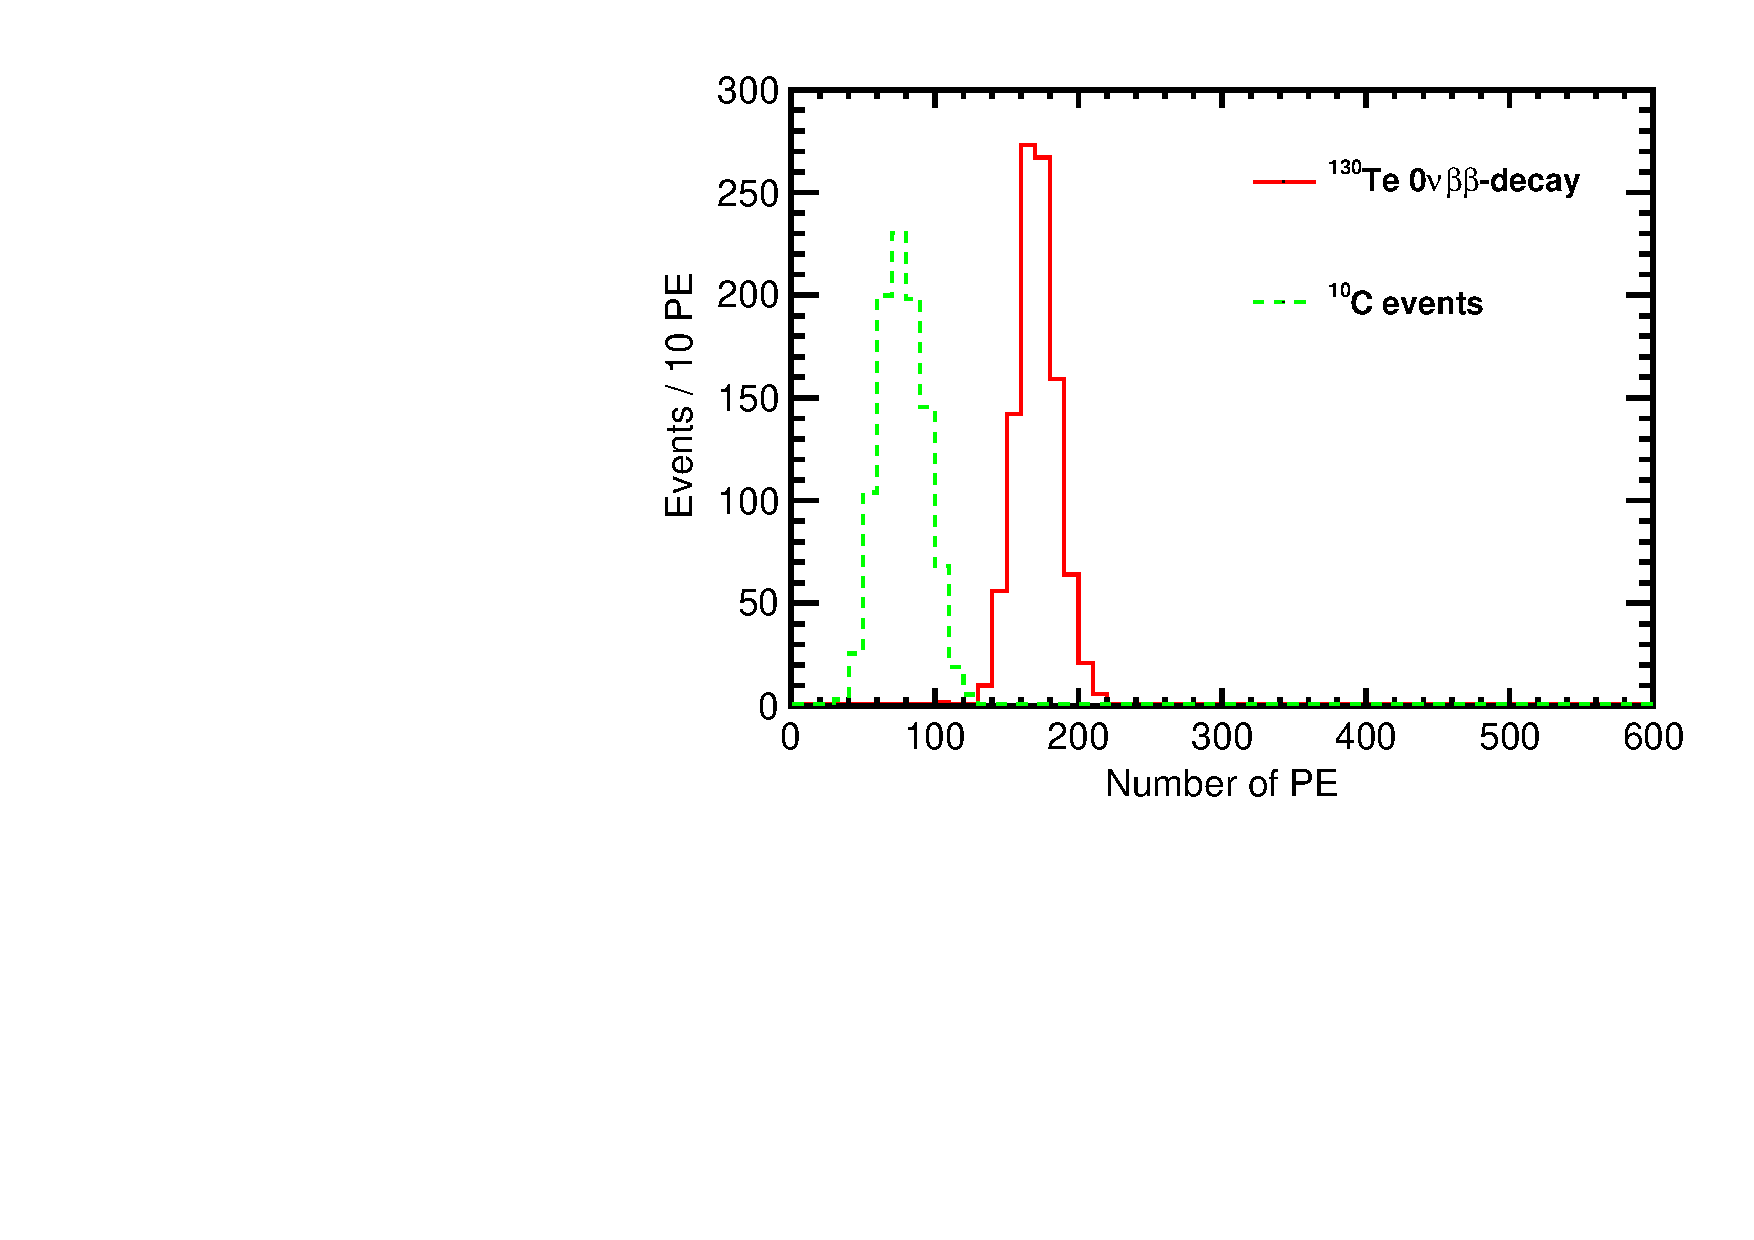
\includegraphics[width=0.45\textwidth]{hMomNPhot_Te130vsC10_allLight_VtxSmear3cm_VtxShiftX0cm_momDT1p0ns_rndVtx_3p0mSphere.pdf}
%  \caption{}
%\label{fig:0nbb-C10_timing_separation}
%\end{figure}

